\chapter{Evaluation}%
\label{cha:evaluation}

%As a rough outline, this chapter should address the following questions:
%\begin{itemize}
%   \item Which questions did you want to answer or which hypothesises did you want to test with the experiments?
%   \item Which metrics did you measure and how does their value relate to the questions you want to answer?
%   \item Which system parameters exist that may have an influence on the value on the metric? Which ones did you vary in your experiments? Intuitively, what are your expectations with regards to the relationship between the system parameters and the metrics?
%   \item How did the experiments that you did actually looked like, or how did you actually measure the chosen metrics?
%   \item What are the actual values that you measured in your experiments? Do they match your intuition about the relationship between the system parameters and the metrics?
%\end{itemize}

%\section{Auswertung der Testergebnisse}

\section{Vergleich der Kontextkategorien} 
%\subsection{Theoretische Mächtigkeit einzelner Kategorien} 
\subsection{Verfügbarkeit der Informationen}
Die Informationen die ich in den definierten Kategorien als gegeben vorausgesetzt habe sind in der Praxis unterschiedlich schwer zu akquirieren. Offensichtlich ist es um ein Vielfaches einfacher korrekt die aktuelle Uhrzeit zu ermitteln als den Grund dafür das ein Nutzer eine Aktion ausführt zu bestimmen. Die nachfolgende Grafik dient dazu den meiner Einschätzung nach benötigten Aufwand zur Beschaffung einer Information zu veranschaulichen.\\
%TODO Grafik
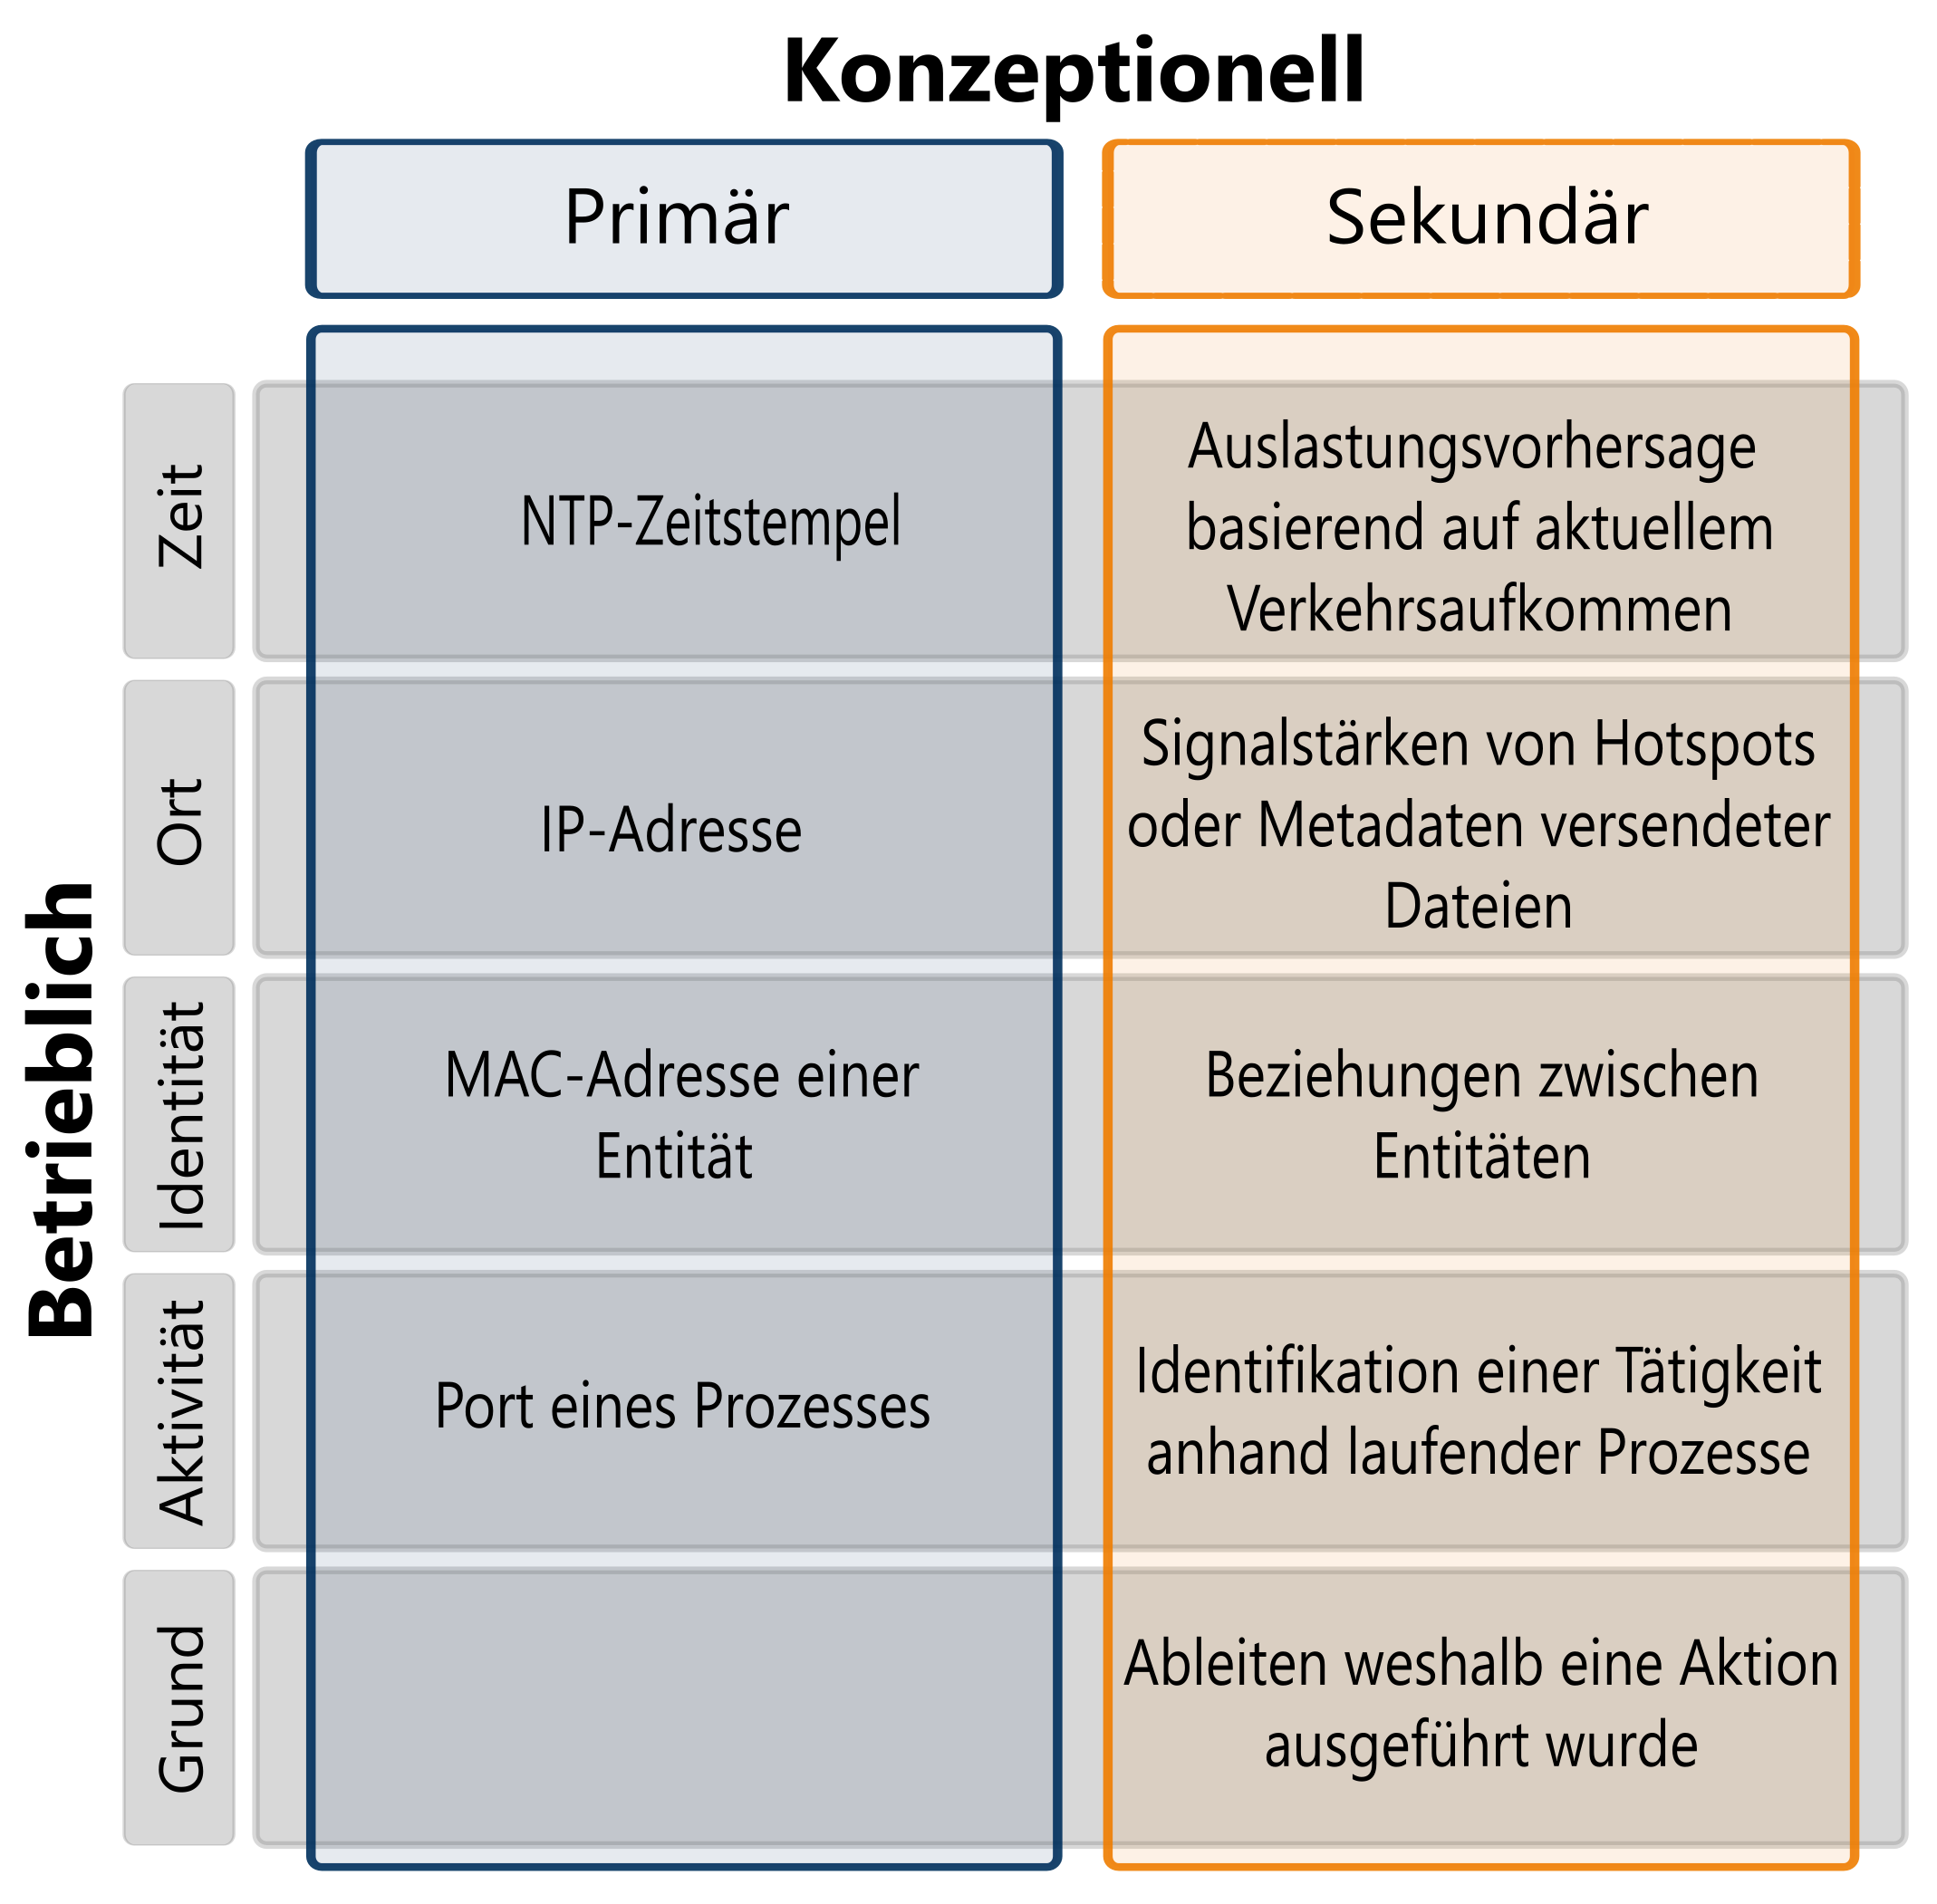
\includegraphics[width=13.5cm,height=12cm]{graphic_1}\\
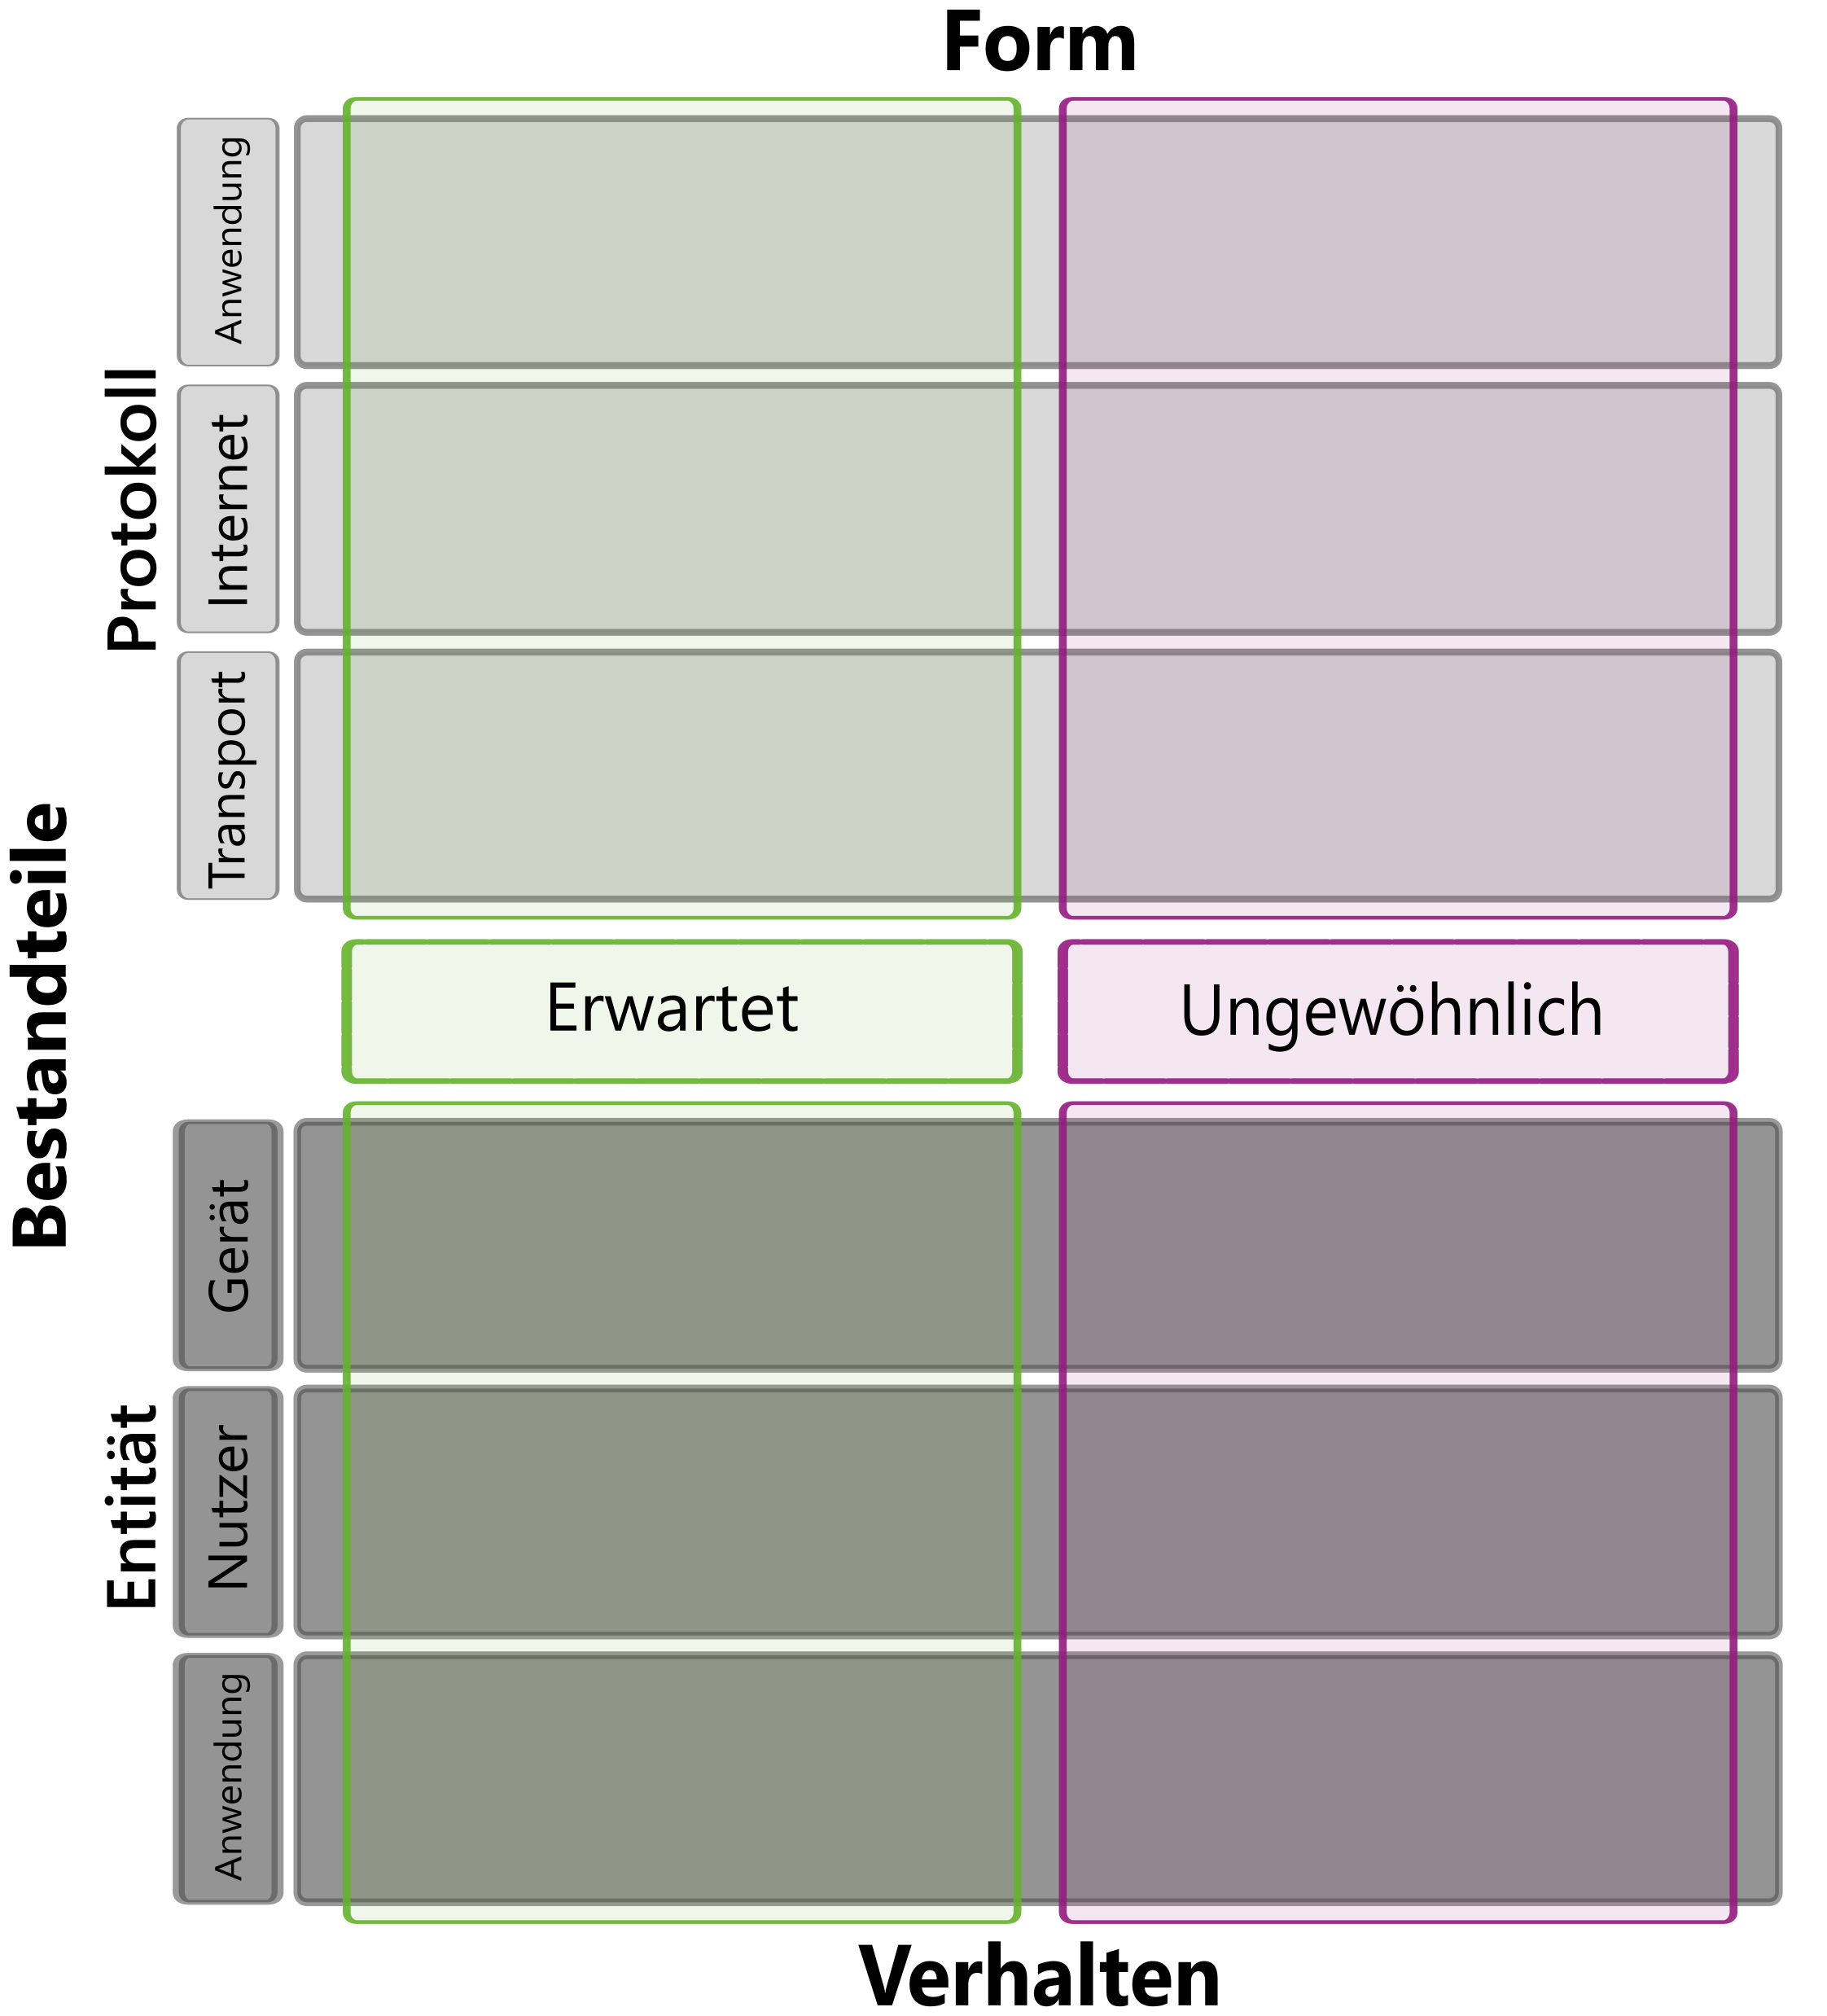
\includegraphics[width=13.5cm,height=13cm]{graphic_2}\pagebreak
\subsection{Qualität der Informationen}
Auch die Qualität der Informationen schwankt in der Praxis. Genauigkeit und Korrektheit der Informationen sind teils unterschiedlich. Auch die Vertrauenswürdigkeit und Aktualität der Aquirierungspunkte ist verschieden.
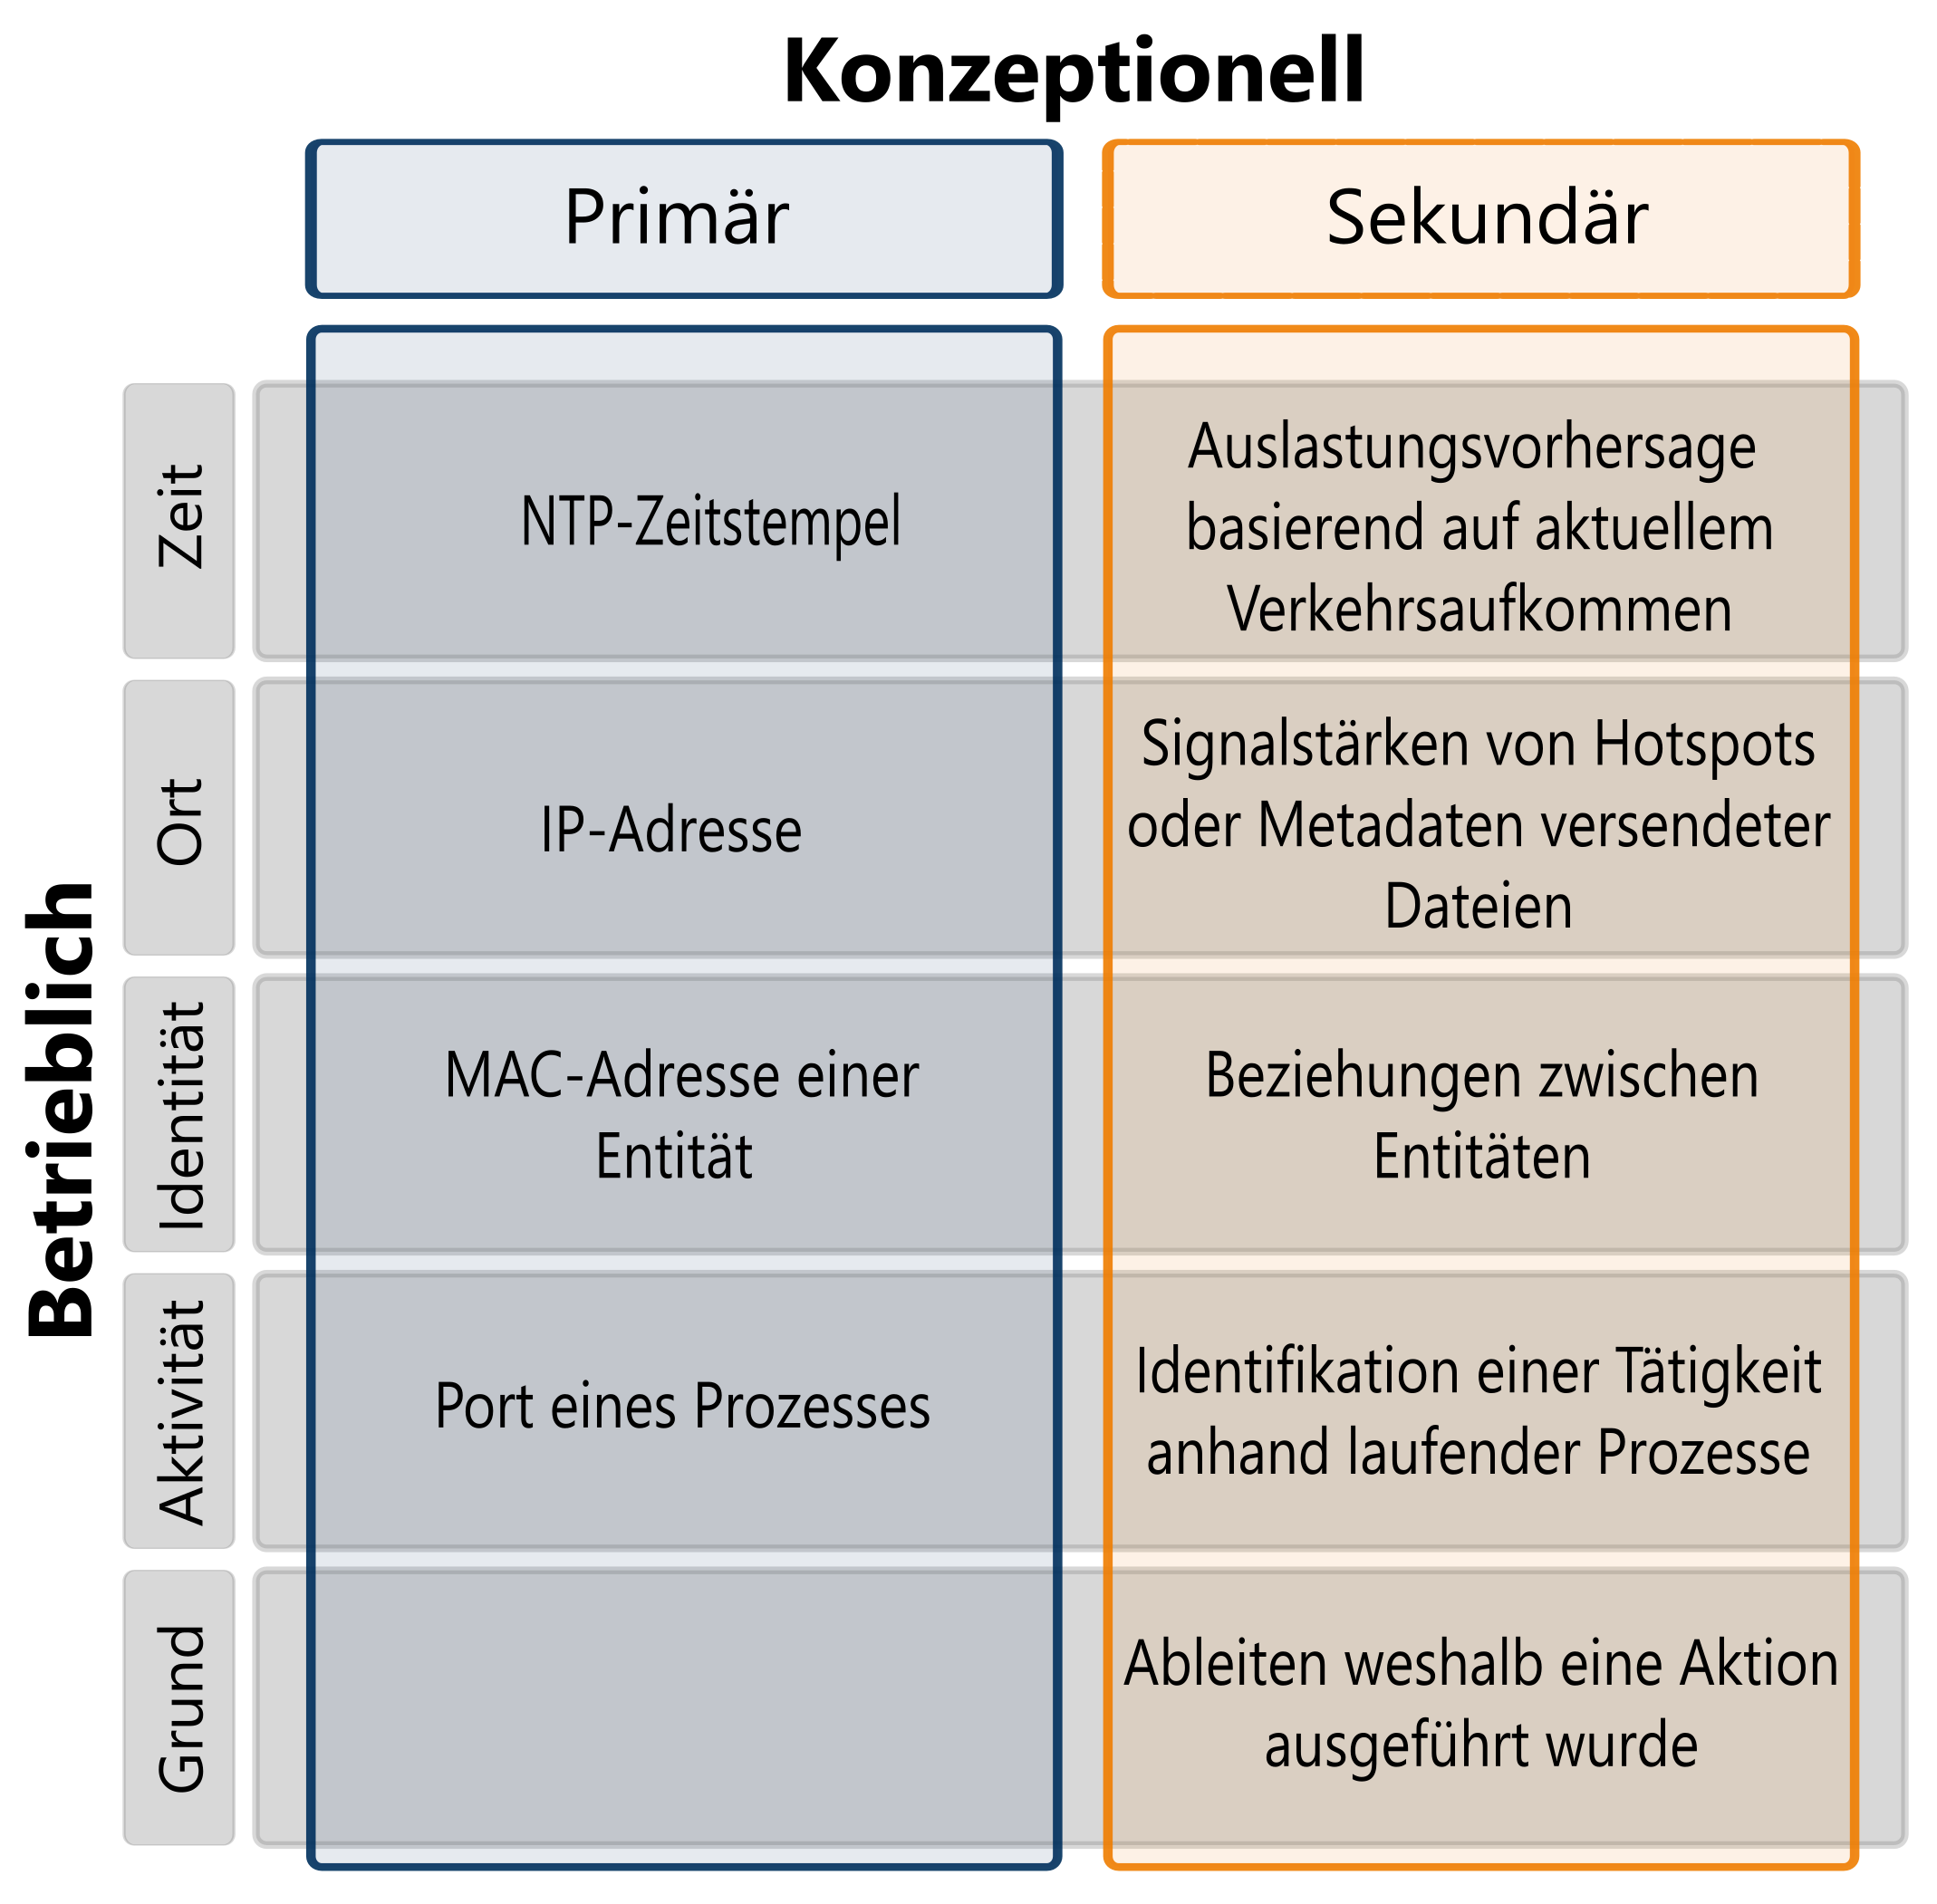
\includegraphics[width=13.5cm,height=12cm]{graphic_1}\\
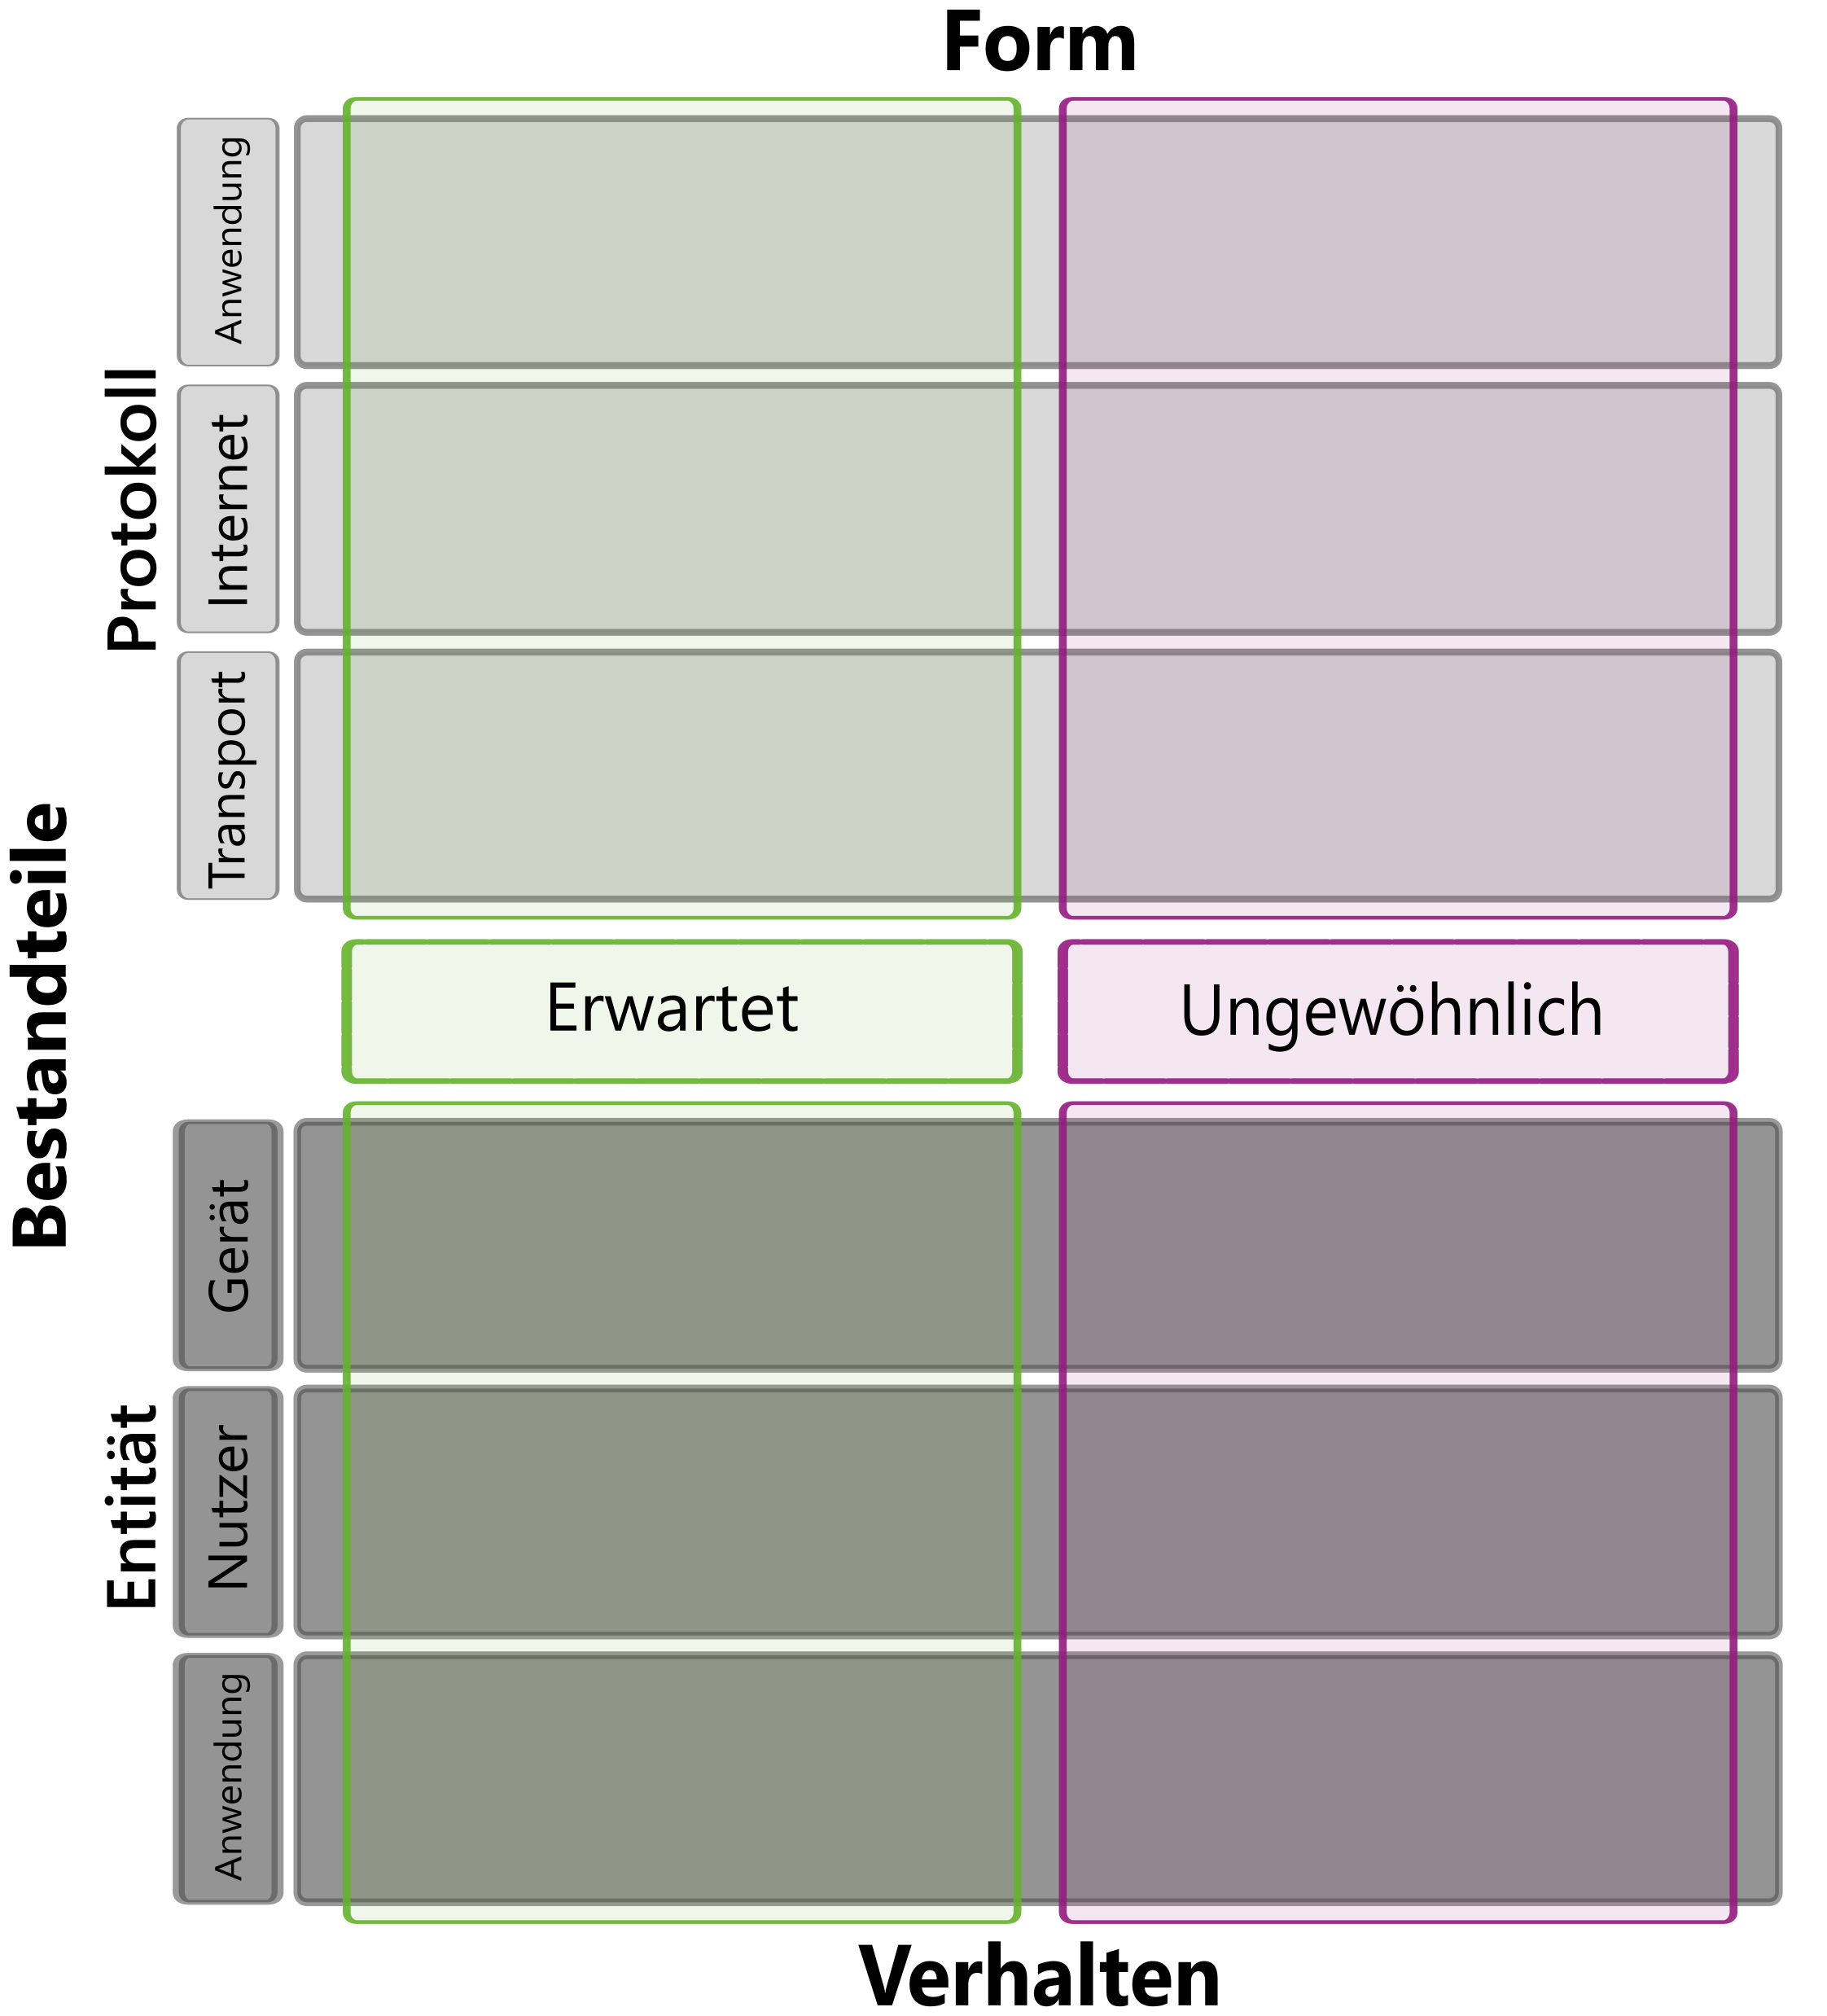
\includegraphics[width=13.5cm,height=13cm]{graphic_2}
\pagebreak

\section{Erhöhung der Netzwerksicherheit}
\subsection{Nicht-kontextsensitive Signaturen}
\subsection{Kontextsensitive Signaturen} 
